\documentclass[11pt]{article}
\usepackage[margin=1in]{geometry}
\usepackage{amsmath,amssymb,amsthm,mathtools}
\usepackage{graphicx}
\usepackage{microtype}
\usepackage[hidelinks]{hyperref}
\usepackage{tikz}

\newtheorem{theorem}{Theorem}
\newtheorem{lemma}[theorem]{Lemma}
\newtheorem{corollary}[theorem]{Corollary}
\newcommand{\Sstate}{\mathcal S}
\newcommand{\Eaff}{E(K)}

\title{A stadium spectral effect algebra with\\non-singleton atomic faces}
\author{Counterexample packet for arXiv:1811.12407}
\date{9 August 2026}

\begin{document}
\maketitle

\begin{center}
\fbox{\parbox{0.91\textwidth}{\textbf{Status.}
Likely-valid full negative answers to open questions 1 and 5, pending
human review.  The counterexample is finite-dimensional and explicit.}}
\end{center}

\section{Questions answered}

Jen\v{c}ov\'a and Pl\'avala ask in Questions 1 and 5 on p.~11 of
\cite{JP} whether the extreme states of a spectral effect algebra have the
atomic exposed form, and whether
\[
 \widehat a=\{s\in\Sstate(E):s(a)=1\}
\]
is a singleton for every sharp one-dimensional effect
$a\in S_1(E)$.  Both answers are \emph{no}.

\begin{figure}[ht]
\centering
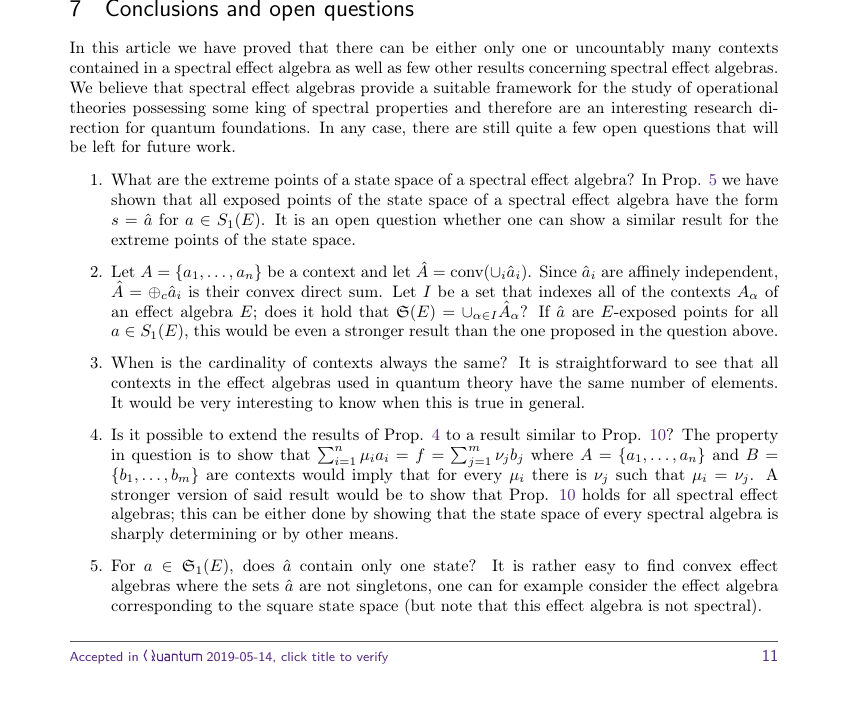
\includegraphics[width=0.94\textwidth]{figures/open_questions_crop.png}
\caption{The source paper's open questions 1--5 \cite[p.~11]{JP}.}
\end{figure}

\section{The stadium and its affine effect algebra}

Let $D$ be the Euclidean unit disk in $\mathbb R^2$, let
$L=[-1,1]\times\{0\}$, and set
\[
 K=L+D.
\]
Thus $K$ is the planar stadium
\begin{equation}\label{eq:stadium}
 K=\left\{(x_1,x_2):
 \bigl(\max\{|x_1|-1,0\}\bigr)^2+x_2^2\leq1\right\}.
\end{equation}
It is a compact centrally symmetric convex body.

Let $E(K)$ be the convex effect algebra of all affine functions
$f:K\to[0,1]$, with unit the constant function $1$.  As recalled in
\cite{JP}, its state space is affinely isomorphic to $K$: a point
$x\in K$ acts by evaluation, $s_x(f)=f(x)$.

\begin{figure}[ht]
\centering
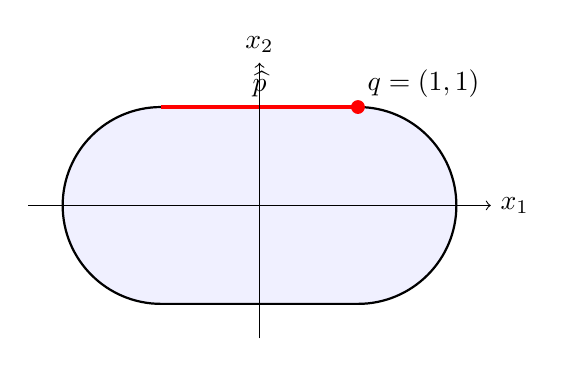
\begin{tikzpicture}[scale=1.25]
  \fill[blue!6] (-1,1)--(1,1)
    arc[start angle=90,end angle=-90,radius=1]
    --(-1,-1) arc[start angle=270,end angle=90,radius=1]--cycle;
  \draw[thick] (-1,1)--(1,1)
    arc[start angle=90,end angle=-90,radius=1]
    --(-1,-1) arc[start angle=270,end angle=90,radius=1]--cycle;
  \draw[very thick,red] (-1,1)--(1,1);
  \fill[red] (1,1) circle (2pt);
  \node[above right] at (1,1) {$q=(1,1)$};
  \node[above] at (0,1) {$\widehat p$};
  \draw[->] (-2.35,0)--(2.35,0) node[right] {$x_1$};
  \draw[->] (0,-1.35)--(0,1.45) node[above] {$x_2$};
\end{tikzpicture}
\caption{The stadium $K$.  The red top segment is the atomic face
$\widehat p$; its endpoint $q$ is extreme but not exposed.}
\end{figure}

For $z=(z_1,z_2)\in(\mathbb R^2)^*$, the support norm of $K$ is
\begin{equation}\label{eq:dualnorm}
 \|z\|_*=\max_{x\in K}z(x)
 =|z_1|+\sqrt{z_1^2+z_2^2}.
\end{equation}
Indeed support functions add under Minkowski sums.  This norm is strictly
convex: equality in its triangle inequality forces equality in the
Euclidean triangle inequality, hence positive collinearity; two unit
vectors with that property are equal.

\section{Why the effect algebra is spectral}

We record the elementary mechanism in a form that also verifies every
effect-algebra detail needed by the counterexample.

\begin{lemma}[Two-context spectrality]\label{lem:spectral}
Let $K$ be a compact centrally symmetric convex body whose support norm
$\|\cdot\|_*$ on the dual space is strictly convex.  Then $E(K)$ is a
spectral effect algebra.  More precisely, for every $\|y\|_*=1$,
\[
 p_y(x)=\frac{1+y(x)}2,\qquad p_{-y}=1-p_y
\]
are sharp one-dimensional effects, so $\{p_y,p_{-y}\}$ is a context, and
every effect is a linear combination of such a context with coefficients
in $[0,1]$.
\end{lemma}

\begin{proof}
Identify an affine function with a pair $(\alpha,z)$ via
$f(x)=\alpha+z(x)$.  Central symmetry gives
\[
 f\geq0\ \Longleftrightarrow\ \alpha\geq\|z\|_*,
 \qquad
 0\leq f\leq1\ \Longleftrightarrow\
 \|z\|_*\leq\min\{\alpha,1-\alpha\}.
\]

Fix $\|y\|_*=1$ and suppose $0\leq g=(\beta,w)\leq
p_y=(1/2,y/2)$.  Then
\[
 \|w\|_*\leq\beta,\qquad
 \|y/2-w\|_*\leq\tfrac12-\beta.
\]
Consequently,
\[
 \tfrac12=\|y/2\|_*
 \leq\|w\|_*+\|y/2-w\|_*
 \leq\beta+\tfrac12-\beta=\tfrac12.
\]
All inequalities are equalities.  Strict convexity makes $w$ and
$y/2-w$ nonnegative collinear, and the two displayed bounds then give
$g=\lambda p_y$ for some $\lambda\in[0,1]$.  Thus $p_y$ is
one-dimensional.  If also $g\leq1-p_y$, choose $x\in K$ with $y(x)=1$.
Then $g(x)=\lambda$ while $(1-p_y)(x)=0$, so $\lambda=0$.
Therefore $p_y$ is sharp.  The same applies to $p_{-y}$, and their sum is
$1$.

Finally let $f=(\alpha,z)\in E(K)$ and put $r=\|z\|_*$.  If $r>0$, set
$y=z/r$; if $r=0$, choose any dual unit vector $y$.  Since
$r\leq\min\{\alpha,1-\alpha\}$,
\[
 \mu=\alpha+r,\qquad \nu=\alpha-r
\]
belong to $[0,1]$, and direct calculation gives
\[
 f=\mu p_y+\nu p_{-y}.
\]
This is a spectral decomposition over the context
$\{p_y,p_{-y}\}$.
\end{proof}

Equation \eqref{eq:dualnorm} and Lemma~\ref{lem:spectral} show that the
stadium effect algebra $E(K)$ is spectral in exactly the finite-context
sense used in the source paper.

\section{The two negative answers}

\begin{theorem}[Non-singleton atomic face]\label{thm:q5}
Question 5 of \cite{JP} has a negative answer.  In the spectral effect
algebra $E(K)$, the effect
\[
 p(x_1,x_2)=\frac{1+x_2}{2}
\]
belongs to $S_1(E(K))$, but $\widehat p$ is not a singleton.
\end{theorem}

\begin{proof}
The functional $y(x_1,x_2)=x_2$ has $\|y\|_*=1$, so
Lemma~\ref{lem:spectral} gives $p=p_y\in S_1(E(K))$.  Under the
evaluation identification $\Sstate(E(K))=K$,
\[
 \widehat p=\{x\in K:p(x)=1\}
 =[-1,1]\times\{1\},
\]
the whole top line segment of the stadium.
\end{proof}

\begin{theorem}[Extreme need not be exposed]\label{thm:q1}
Question 1 of \cite{JP} also has a negative answer.  The state
$q=(1,1)\in K=\Sstate(E(K))$ is extreme, but it is not exposed and hence
cannot have the form $\widehat a=\{q\}$ for any $a\in S_1(E(K))$.
\end{theorem}

\begin{proof}
If $q=(x+x')/2$ with $x,x'\in K$, then both second coordinates are at
most $1$ and average to $1$, so both equal $1$.  Formula
\eqref{eq:stadium} then puts both first coordinates in $[-1,1]$; since
their average is $1$, both equal $1$.  Thus $x=x'=q$, proving
extremality.

For non-exposedness, write $K=L+D$.  If a nonzero functional
$z=(z_1,z_2)$ is maximized at $q=(1,0)+(0,1)$, then $(0,1)$ must maximize
$z$ over the Euclidean disk.  Hence $z$ is a positive multiple of
$(0,1)$.  But that functional is maximized on all of
$[-1,1]\times\{1\}$, not uniquely at $q$.  Therefore $q$ is not exposed.
If $\widehat a=\{q\}$ for an effect $a$, then $a$ itself would expose
$q$ by its maximum value $1$, a contradiction.
\end{proof}

\section{Checks, scope, and novelty}

The construction is two-dimensional; no closure, completeness, or
infinite-sum issue is hidden.  The proof directly checks the source
definition of a context and gives a spectral decomposition of every affine
effect.  The square mentioned in the source fails because its support norm
is not strictly convex.  Rounding the square's left and right sides into
tangent semicircles makes the dual norm strictly convex while deliberately
retaining the top and bottom faces.

This packet fully answers Questions 1 and 5 negatively.  It does not settle
Questions 2--4 or the broad weak-duality Question 6.

A bounded search through 9 August 2026 used the source title and exact
question language together with the phrases \emph{spectral effect algebra},
\emph{singleton atomic face}, \emph{centrally symmetric state space}, and
\emph{stadium}.  No explicit answer by this counterexample was found.
Subsequent work of Jen\v{c}ov\'a and Pulmannov\'a \cite{JPU} studies
centrally symmetric state spaces and characterizes related, but differently
formulated, compression-base notions of spectrality.  That paper makes the
Banach-space geometry strongly adjacent, so novelty confidence is
\emph{moderate to low}; the present packet's contribution is the direct
finite-context calculation and its explicit application to the two 2019
questions.

\paragraph{Human-review recommendation.}
Check the equivalence between point evaluations and states of $E(K)$, the
one-dimensionality equality case in Lemma~\ref{lem:spectral}, and whether
\cite{JPU} or later citing work explicitly records the same answers before
making a novelty claim.

\begin{thebibliography}{9}
\bibitem{JP}
A. Jen\v{c}ov\'a and M. Pl\'avala,
\emph{On the properties of spectral effect algebras},
Quantum 3 (2019), 148,
\href{https://doi.org/10.22331/q-2019-06-03-148}{doi:10.22331/q-2019-06-03-148};
\href{https://arxiv.org/abs/1811.12407}{arXiv:1811.12407}.

\bibitem{JPU}
A. Jen\v{c}ov\'a and S. Pulmannov\'a,
\emph{Geometric and algebraic aspects of spectrality in order unit spaces:
a comparison},
J. Math. Anal. Appl. 504 (2021), 125360,
\href{https://doi.org/10.1016/j.jmaa.2021.125360}{doi:10.1016/j.jmaa.2021.125360};
\href{https://arxiv.org/abs/2102.01628}{arXiv:2102.01628}.
\end{thebibliography}

\end{document}
